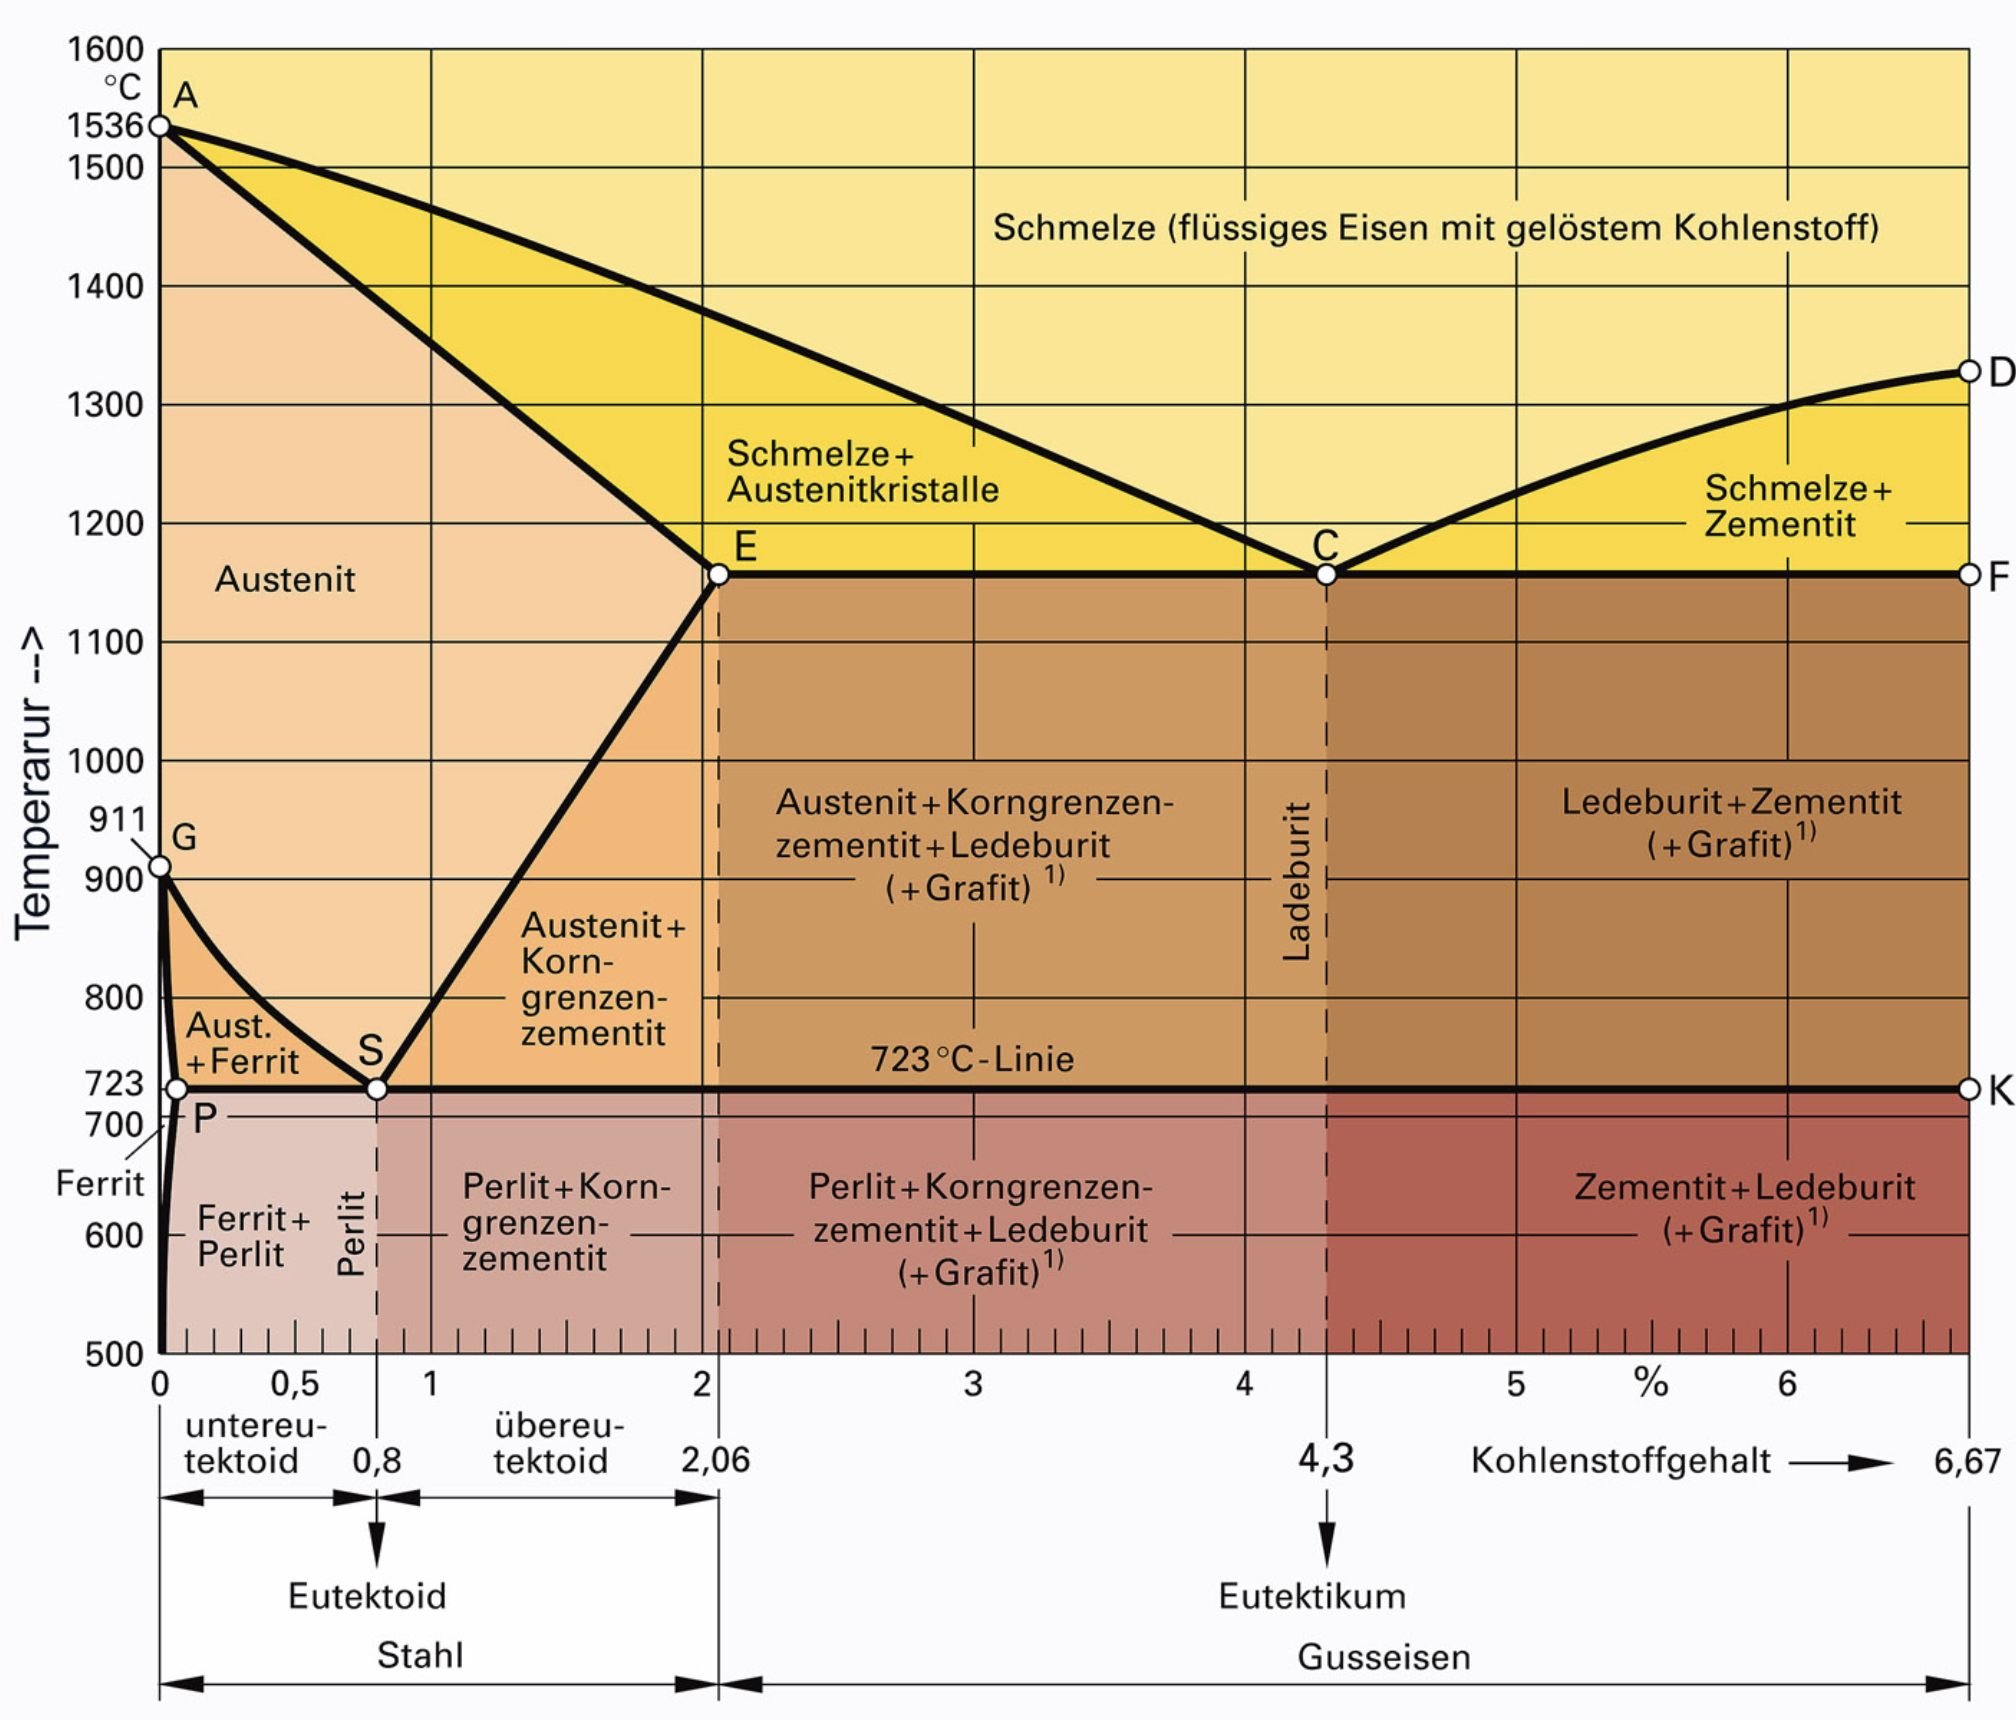
\includegraphics[width = 70mm]{src/images/Eisenkohlenstoffdiagramm.png}
\begin{minipage}{0.39\linewidth}
    \begin{itemize}
        \item Austenit = $\gamma$\\
        \item Ferrit = $\alpha$\\
        \item Zementit = $Fe_3C$\\
    \end{itemize}
\end{minipage}
\begin{minipage}{0.62\linewidth}
    \begin{itemize}
        \item Perlit = Ferrit + Zementit\\
        \item Ledeburit I = Austenit + Zementit\\
        \item Ledeburit II = Perlit + Zementit\\    
    \end{itemize}
\end{minipage}

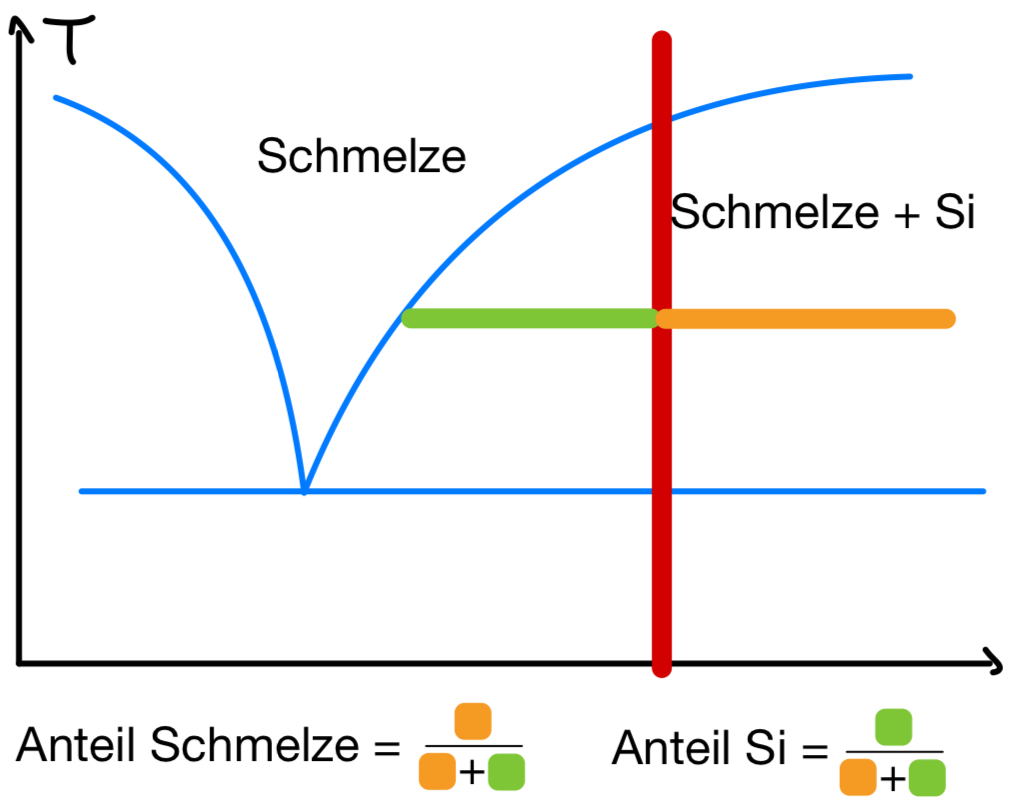
\includegraphics[width = 70mm]{src/images/Hebelgesetz.jpeg}

\begin{minipage}{0.6\linewidth}
    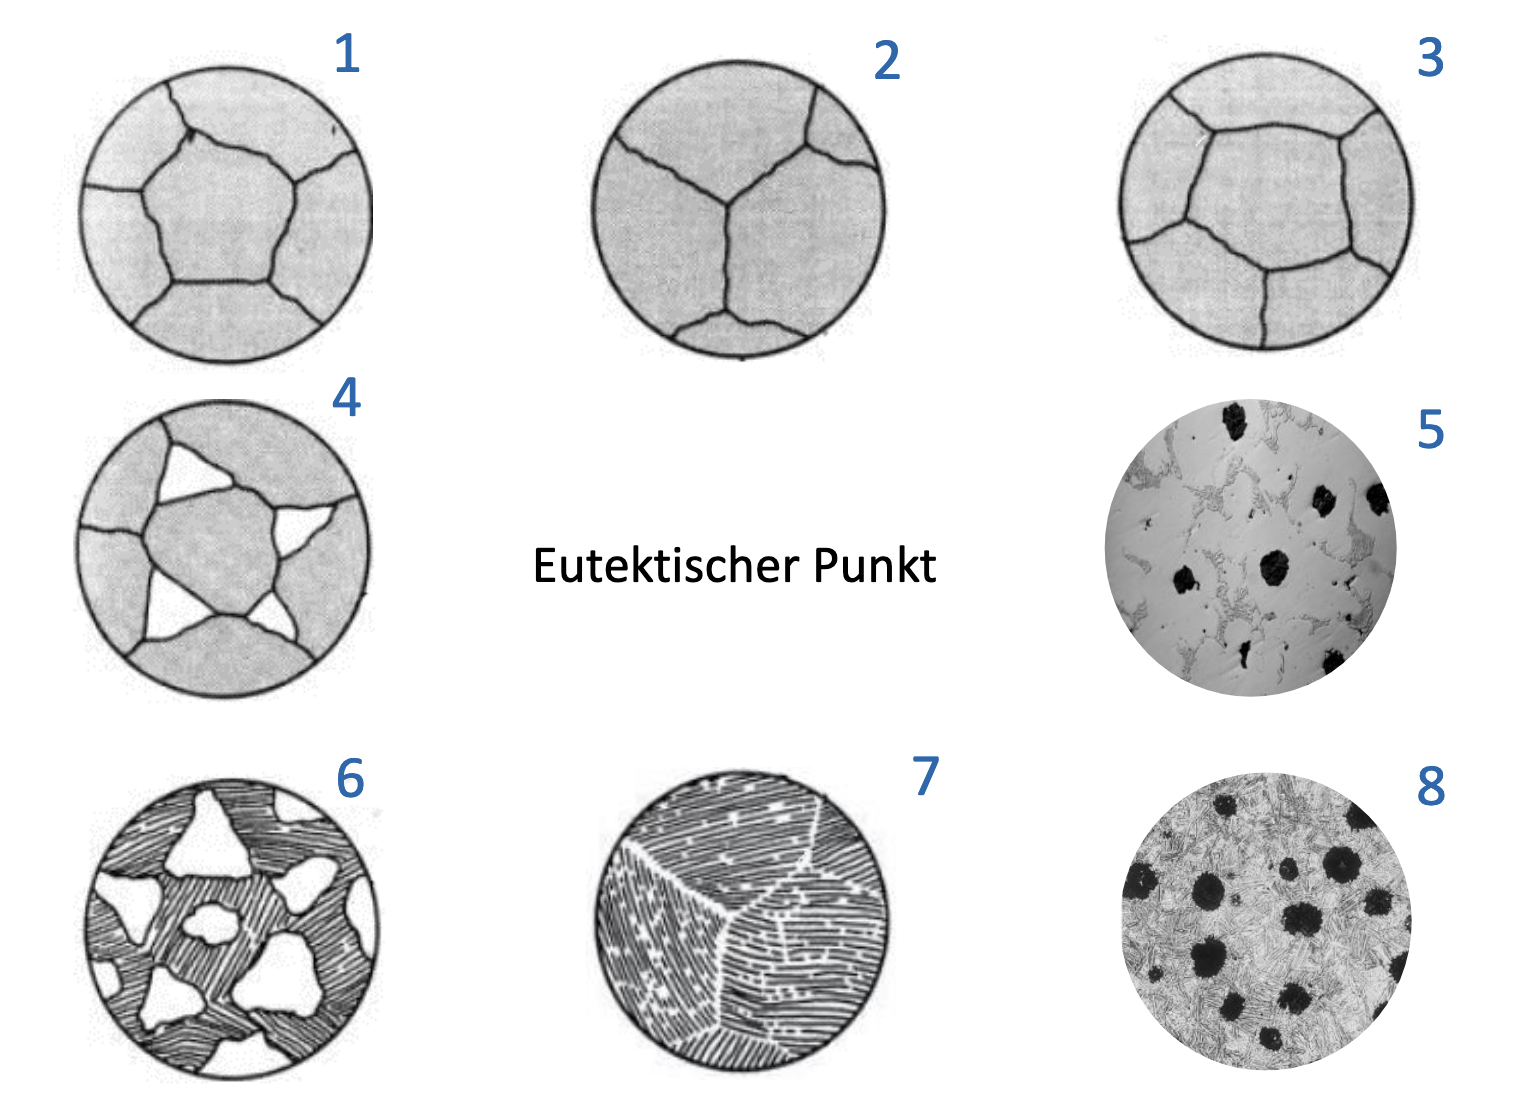
\includegraphics[width = 40mm]{src/images/Kreisli.png}
\end{minipage}
\begin{minipage}{0.4\linewidth}
    1 - 3: Austenit\\
    4: Austenit + Ferrit\\
    5: Austenit + Graphit\\
    6: Perlit + Ferrit\\
    7: Perlit\\
    8: Perlit + Graphit\\
\end{minipage}

